\documentclass{beamer}
\usepackage[utf8]{inputenc}
\usepackage{graphicx, epsfig}
\usepackage{amsmath,mathrsfs,amsfonts,amssymb}
\usepackage{floatflt}
\usepackage{epic,ecltree}
\usepackage{mathtext}
\usepackage{fancybox}
\usepackage{fancyhdr}
\usepackage{multirow}
\usepackage{enumerate}
\usepackage{epstopdf}
\usepackage{multicol}
\usepackage{algorithm}
\usepackage[noend]{algorithmic}
\usepackage{tikz}
\usepackage{blindtext}
\usetheme{default}%{Singapore}%{Warsaw}%{Warsaw}%{Darmstadt}
\usecolortheme{default}

\setbeamerfont{title}{size=\Huge}
\setbeamertemplate{footline}[page number]{}

\setbeamertemplate{section in toc}[sections numbered]


\makeatletter
\newcommand\HUGE{\@setfontsize\Huge{35}{40}}
\makeatother    

\setbeamerfont{title}{size=\HUGE}
\beamertemplatenavigationsymbolsempty

% latin bold lower
\newcommand{\ba}{\mathbf{a}} 
\newcommand{\bc}{\mathbf{c}} 
\newcommand{\be}{\mathbf{e}} 
\newcommand{\bff}{\mathbf{f}} % \bf - for bold type
\newcommand{\bg}{\mathbf{g}} 
\newcommand{\bh}{\mathbf{h}} 
\newcommand{\bp}{\mathbf{p}} 
\newcommand{\bq}{\mathbf{q}} 
\newcommand{\bt}{\mathbf{t}} 
\newcommand{\bs}{\mathbf{s}} 
\newcommand{\bu}{\mathbf{u}} 
\newcommand{\bv}{\mathbf{v}} 
\newcommand{\bw}{\mathbf{w}} 
\newcommand{\bx}{\mathbf{x}} 
\newcommand{\by}{\mathbf{y}} 
\newcommand{\bz}{\mathbf{z}} 

% latin bold upper
\newcommand{\bA}{\mathbf{A}} 
\newcommand{\bB}{\mathbf{B}} 
\newcommand{\bC}{\mathbf{C}} 
\newcommand{\bG}{\mathbf{G}} 
\newcommand{\bI}{\mathbf{I}} 
\newcommand{\bJ}{\mathbf{J}} 
\newcommand{\bL}{\mathbf{L}} 
\newcommand{\bM}{\mathbf{M}} 
\newcommand{\bP}{\mathbf{P}}
\newcommand{\bQ}{\mathbf{Q}} 
\newcommand{\bR}{\mathbf{R}} 
\newcommand{\bT}{\mathbf{T}} 
\newcommand{\bU}{\mathbf{U}} 
\newcommand{\bV}{\mathbf{V}} 
\newcommand{\bW}{\mathbf{W}} 
\newcommand{\bX}{\mathbf{X}} 
\newcommand{\bY}{\mathbf{Y}} 
\newcommand{\bZ}{\mathbf{Z}} 

% latin cal upper
\newcommand{\cF}{\mathcal{F}} 
\newcommand{\cG}{\mathcal{G}} 
\newcommand{\cI}{\mathcal{I}} 
\newcommand{\cL}{\mathcal{L}} 
\newcommand{\cM}{\mathcal{M}} 
\newcommand{\cN}{\mathcal{N}} 
\newcommand{\cP}{\mathcal{P}} 
\newcommand{\cS}{\mathcal{S}} 
\newcommand{\cT}{\mathcal{T}} 
\newcommand{\cW}{\mathcal{W}} 
\newcommand{\cX}{\mathcal{X}} 
\newcommand{\cZ}{\mathcal{Z}} 

% latin bb upper
\newcommand{\bbE}{\mathbb{E}} 
\newcommand{\bbI}{\mathbb{I}} 
\newcommand{\bbP}{\mathbb{P}} 
\newcommand{\bbR}{\mathbb{R}} 

% greek bold lower
\newcommand{\bepsilon}{\boldsymbol{\epsilon}} 
\newcommand{\btheta}{\boldsymbol{\theta}} 
\newcommand{\blambda}{\boldsymbol{\lambda}} 
\newcommand{\bpi}{\boldsymbol{\pi}} 
\newcommand{\bmu}{\boldsymbol{\mu}} 
\newcommand{\bsigma}{\boldsymbol{\sigma}} 
\newcommand{\bphi}{\boldsymbol{\phi}} 

% greek bold upper
\newcommand{\bSigma}{\boldsymbol{\Sigma}} 

\DeclareMathOperator*{\argmin}{arg\,min}
\DeclareMathOperator*{\argmax}{arg\,max}

\newcommand{\createdgmtitle}[1]{\title[\hbox to 56mm{Deep Generative Models  \hfill\insertframenumber\,/\,\inserttotalframenumber}]
	{\vspace{1cm} \\ \textbf{Deep Generative Models} \\ {\Huge Lecture #1}}
	\author{Roman Isachenko}
		\institute{
\includegraphics[width=0.7cm]{../utils/aimasterslogo} \LARGE{AI Masters}}
	\date{2024, Spring}
}

\usepackage{tikz}
\usetikzlibrary{arrows,shapes,positioning,shadows,trees}

\newcommand\myfootnote[1]{%
  \tikz[remember picture,overlay]
  \draw (current page.south west) +(1in + \oddsidemargin,0.5em)
  node[anchor=south west,inner sep=0pt]{\parbox{\textwidth}{%
      \rlap{\rule{10em}{0.4pt}}\raggedright\scriptsize \textit{#1}}};}

\newcommand\myfootnotewithlink[2]{%
  \tikz[remember picture,overlay]
  \draw (current page.south west) +(1in + \oddsidemargin,0.5em)
  node[anchor=south west,inner sep=0pt]{\parbox{\textwidth}{%
      \rlap{\rule{10em}{0.4pt}}\raggedright\scriptsize\href{#1}{\textit{#2}}}};}
      
\AtBeginSection[]
      {
      	\begin{frame}{Outline}
      		\tableofcontents[currentsection]
      	\end{frame}
      }
      \AtBeginSubsection[]{
      	\begin{frame}{Outline}
      		\tableofcontents[currentsection,currentsubsection]
      	\end{frame}
}
\createdgmtitle{8}
%--------------------------------------------------------------------------------
\begin{document}
%--------------------------------------------------------------------------------
\begin{frame}[noframenumbering,plain]
%\thispagestyle{empty}
\titlepage
\end{frame}
%=======
\begin{frame}{Recap of previous lecture}
	\begin{itemize}
		\item Standard Gaussian $p(\bz) = \mathcal{N}(0, \bI)$ $\Rightarrow$ over-regularization;
		\item $p(\bz) = q_{\text{agg}}(\bz | \bphi) = \frac{1}{n}\sum_{i=1}^n q(\bz | \bx_i, \bphi)$ $\Rightarrow$ overfitting and highly expensive.
	\end{itemize}
	\begin{block}{ELBO revisiting}
		\vspace{-0.4cm}
		\[
		\frac{1}{n}\sum_{i=1}^n \cL_{\bphi, \btheta}(\bx_i) = \text{RL} - \text{MI} -  KL(q_{\text{agg}}(\bz | \bphi) || {\color{violet}p(\bz | \blambda)})
		\]
		It is Forward KL with respect to $p(\bz | \blambda)$.
	\end{block}
	\begin{block}{ELBO with flow-based VAE prior}
		\vspace{-0.6cm}
		{\small
			\begin{multline*}
				\cL_{\bphi, \btheta}(\bx) = \mathbb{E}_{q(\bz | \bx, \bphi)} \left[ \log p(\bx | \bz, \btheta) + {\color{violet}\log p(\bz | \blambda)} - \log q(\bz | \bx, \bphi) \right] \\
				= \mathbb{E}_{q(\bz | \bx, \bphi)} \Bigl[ \log p(\bx | \bz, \btheta) + \underbrace{ \Bigl({\color{violet} \log p(f_{\blambda}(\bz)) + \log \left| \det (\bJ_\bff) \right|} \Bigr) }_{\text{flow-based prior}} - \log q(\bz | \bx, \bphi) \Bigr] 
			\end{multline*}
		}
		\vspace{-0.5cm}
		\[
		\bz = \bff^{-1}_{\blambda}(\bz^*) = \bg_{\blambda}(\bz^*), \quad \bz^* \sim p(\bz^*) = \cN(0, \bI)
		\]
	\end{block}
	\vspace{-0.5cm}
	\myfootnotewithlink{https://arxiv.org/abs/1611.02731}{Chen X. et al. Variational Lossy Autoencoder, 2016}
\end{frame}
%=======
\begin{frame}{Recap of previous lecture}
	\begin{block}{Likelihood-free learning}
		\begin{itemize}
			\item Likelihood is not a perfect quality measure for generative model.
			\item Likelihood could be intractable.
		\end{itemize}
	\end{block}
	Imagine we have two sets of samples 
	\begin{itemize}
		\item $\cS_1 = \{\bx_i\}_{i=1}^{n_1} \sim \pi(\bx)$ -- real samples;
		\item $\cS_2 = \{\bx_i\}_{i=1}^{n_2} \sim p(\bx | \btheta)$ -- generated (or fake) samples.
	\end{itemize}
	Let define discriminative model (classifier):
	\[
		p(y = 1 | \bx) = P\bigl(\{\bx \sim \pi(\bx)\}\bigr); \quad p(y = 0 | \bx) = P\bigl(\{\bx \sim p(\bx | \btheta)\}\bigr)
	\]
	\vspace{-0.5cm}
	\begin{block}{Assumption}
		Generative distribution $p(\bx | \btheta)$ equals to the true distribution $\pi(\bx)$ if we can not distinguish them using discriminative model $p(y | \bx)$. \\
		It means that $p(y = 1 | \bx) = 0.5$ for each sample $\bx$.
	\end{block}
\end{frame}
%=======
\begin{frame}{Recap of previous lecture}
	\begin{itemize}
		\item \textbf{Generator:} generative model $\bx = \bG(\bz)$, which makes generated sample more realistic.
		\item \textbf{Discriminator:} a classifier $D(\bx) \in [0, 1]$, which distinguishes real samples from generated samples.
	\end{itemize}
	\vspace{-0.1cm}
	\begin{block}{GAN optimality theorem}
		The minimax game 
		\vspace{-0.3cm}
		\[
		\min_{G} \max_D \Bigl[ \underbrace{\bbE_{\pi(\bx)} \log D(\bx) + \bbE_{p(\bz)} \log (1 - D(\bG(\bz)))}_{V(G, D)} \Bigr]
		\]
		\vspace{-0.5cm} \\
		has the global optimum $\pi(\bx) = p(\bx | \btheta)$, in this case $D^*(\bx) = 0.5$.
	\end{block}
	\[
		\min_{G} V(G, D^*) = \min_{G} \left[ 2 JSD(\pi || p) - \log 4 \right] = -\log 4, \quad \pi(\bx) = p(\bx | \btheta).
	\]
	\vspace{-0.5cm} \\
	If the generator could be \textbf{any} function and the discriminator is \textbf{optimal} at every step, then the generator is \textbf{guaranteed to converge} to the data distribution.
	 \myfootnotewithlink{https://arxiv.org/abs/1406.2661}{Goodfellow I. J. et al. Generative Adversarial Networks, 2014}
\end{frame}
%=======
\begin{frame}{Recap of previous lecture}
	\begin{itemize}
		\item Generator updates are made in parameter space, discriminator is not optimal at every step.
		\item Generator and discriminator loss keeps oscillating during GAN training.
	\end{itemize}
	\begin{block}{Objective}
		\vspace{-0.5cm}
		\[
		\min_{\btheta} \max_{\bphi} \left[ \bbE_{\pi(\bx)} \log D_{\bphi}(\bx) + \bbE_{p(\bz)} \log (1 - D_{\bphi}(\bG_{\btheta}(\bz))) \right]
		\]
		\vspace{-0.5cm}
	\end{block}
	\begin{figure}
		\centering
		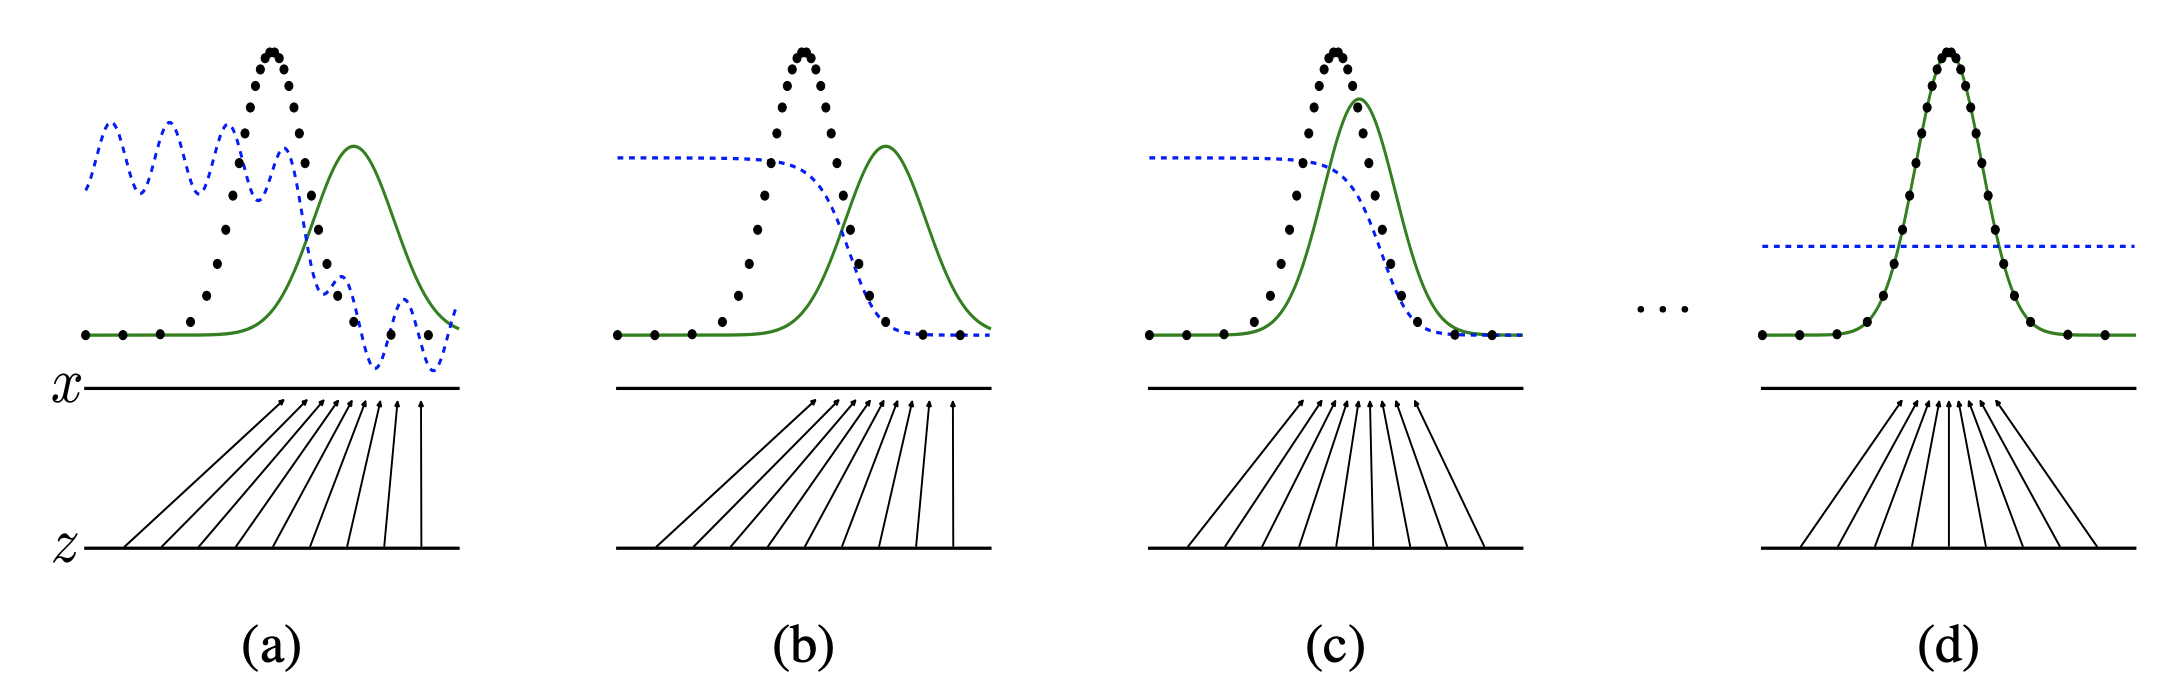
\includegraphics[width=1.0\linewidth]{figs/gan_1}
	\end{figure}
	\myfootnotewithlink{https://arxiv.org/abs/1406.2661}{Goodfellow I. J. et al. Generative Adversarial Networks, 2014}
\end{frame}
%=======
\begin{frame}{Outline}
	\tableofcontents
\end{frame}
%=======
\section{Wasserstein distance}
%=======
\begin{frame}{Informal theoretical results}
	\vspace{-0.3cm}
	\begin{itemize}
		\item The dimensionality of $\bz$ is lower than the dimensionality of $\bx$. Hence, support of $p(\bx | \btheta)$ with $\bx = \bG_{\btheta}(\bz)$ lies on low-dimensional manifold.
		\item Distribution of real images $\pi(\bx)$ is also concentrated on a low dimensional manifold.
		\begin{figure}
			\centering
			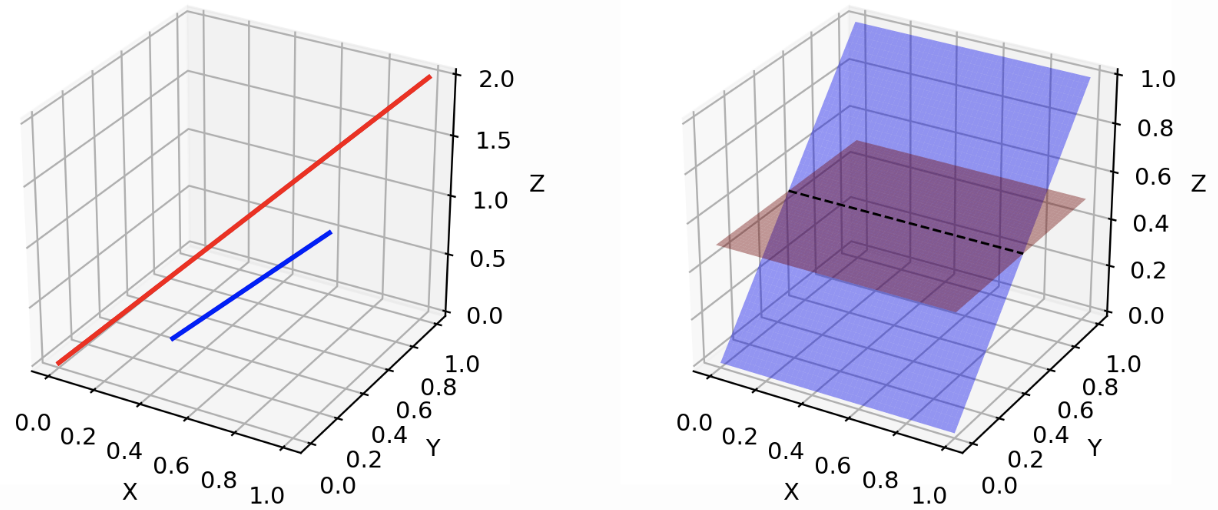
\includegraphics[width=0.55\linewidth]{figs/low_dim_manifold}
		\end{figure}
		\item If $\pi(\bx)$ and $p(\bx | \btheta)$ have disjoint supports, then there is a smooth optimal discriminator.
		\item For such low-dimensional disjoint manifolds
		\vspace{-0.2cm}
		\[
		KL(\pi || p) = KL(p || \pi) = \infty, \quad JSD(\pi || p) = \log 2
		\]
	\end{itemize}
	\myfootnote{\href{https://arxiv.org/abs/1904.08994}{Weng L. From GAN to WGAN, 2019} \\ 
		\href{https://arxiv.org/abs/1701.04862}{Arjovsky M., Bottou L. Towards Principled Methods for Training Generative Adversarial Networks, 2017}}
\end{frame}
%=======
\begin{frame}{Wasserstein distance (discrete)}
	A.k.a. \textbf{Earth Mover's distance}.
	\begin{block}{Optimal transport formulation}
		The minimum cost of moving and transforming a pile of dirt in the shape of one probability distribution to the shape of the other distribution.
	\end{block}
	\begin{figure}
		\centering
		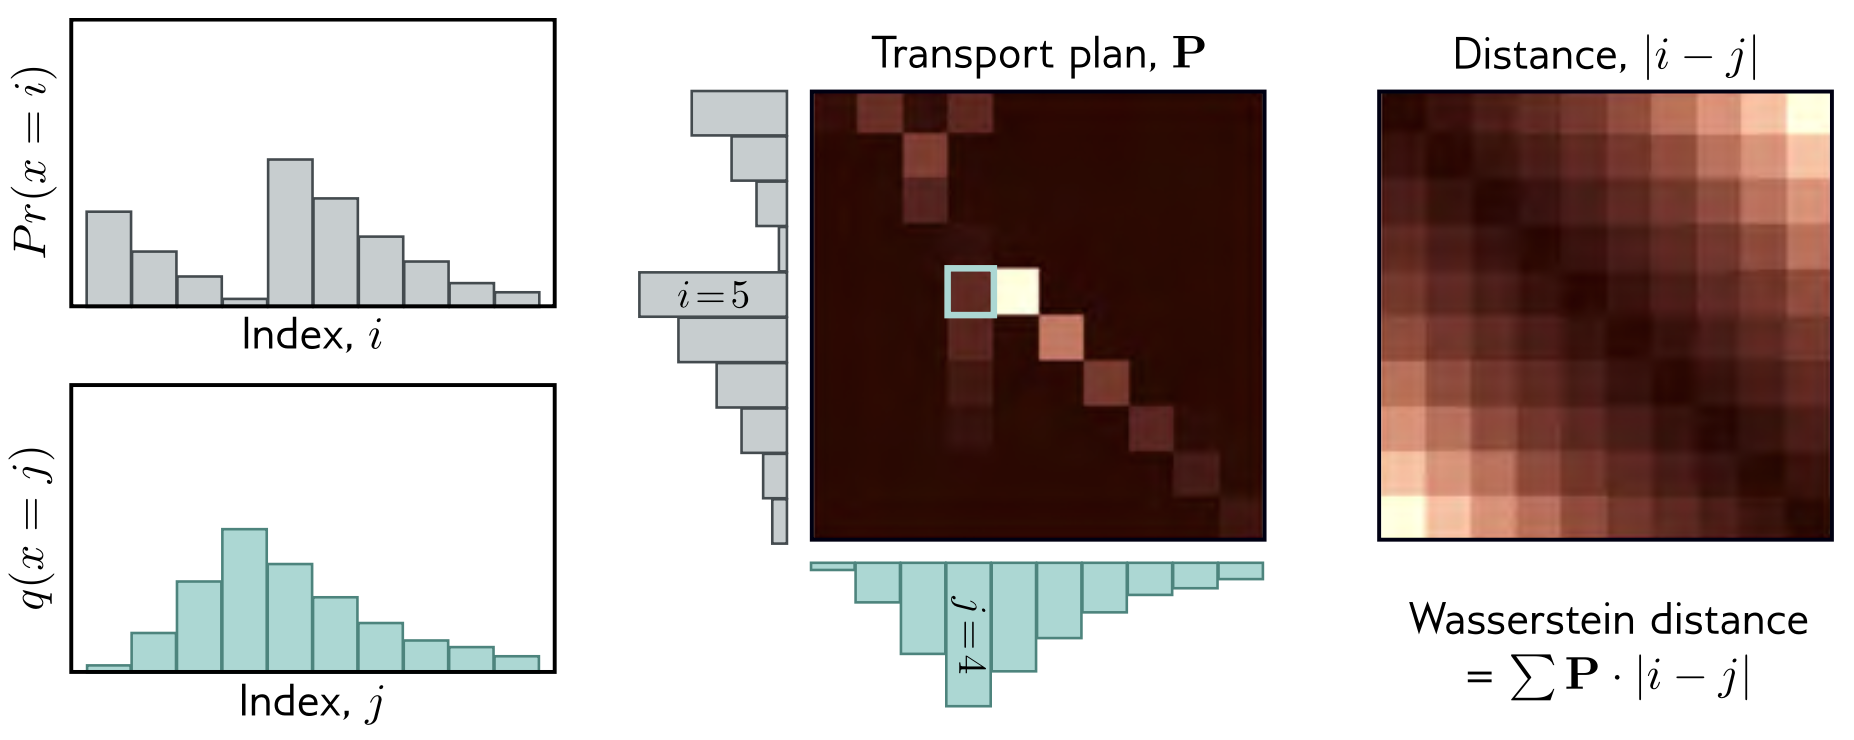
\includegraphics[width=\linewidth]{figs/discrete_wasserstein}
	\end{figure}
	\myfootnotewithlink{https://udlbook.github.io/udlbook/}{Simon J.D. Prince. Understanding Deep Learning, 2023}
\end{frame}
%=======
\begin{frame}{Wasserstein distance (continuous)}
	\vspace{-0.7cm}
	\[
	W(\pi, p) = \inf_{\gamma \in \Gamma(\pi, p)} \bbE_{(\bx, \by) \sim \gamma} \| \bx - \by \| =  \inf_{{\color{olive}\gamma}\in {\color{teal}\Gamma(\pi, p)}} \int {\color{violet} \| \bx - \by \|} {\color{olive}\gamma (\bx, \by)} d \bx d \by
	\]
	\vspace{-0.4cm}
	\begin{itemize}
		\item ${\color{olive}\gamma (\bx, \by)}$ -- transportation plan (the amount of "dirt" that should be transported from point $\bx$ to point $\by$)
		\vspace{-0.2cm}
		\[
		\int \gamma(\bx, \by) d \bx = p(\by); \quad \int \gamma(\bx, \by) d \by = \pi(\bx).
		\]
		\vspace{-0.6cm}
		\item ${\color{teal}\Gamma(\pi, p)}$ -- the set of all joint distributions $\gamma (\bx, \by)$ with marginals $\pi$ and $p$.
		\item ${\color{olive}\gamma(\bx, \by)}$ -- the amount, ${\color{violet} \| \bx - \by \|}$-- the distance.
	\end{itemize}
	\begin{block}{Wasserstein metric}
		\vspace{-0.2cm}
		\[
		W_s(\pi, p) = \inf_{\gamma \in \Gamma(\pi, p)} \left(\bbE_{(\bx, \by) \sim \gamma} \| \bx - \by \|^s\right)^{1/s}
		\]
		\vspace{-0.4cm}
	\end{block}
	Here we will use $W(\pi, p) = W_1(\pi, p)$ that corresponds to the optimal transport formulation.
	\myfootnotewithlink{https://arxiv.org/abs/1701.07875}{Arjovsky M., Chintala S., Bottou L. Wasserstein GAN, 2017}
\end{frame}
%=======
\begin{frame}{Wasserstein distance vs KL vs JSD}
	
	\begin{minipage}[t]{0.48\columnwidth}
		\vspace{0.1cm}
		Consider 2d distributions
		\[
		\pi(x, y) = (0, U[0,1])
		\]	
		\[
		p(x, y | \theta) = (\theta, U[0, 1])
		\]
	\end{minipage}%
	\begin{minipage}[t]{0.52\columnwidth}
		\begin{figure}
			\centering
			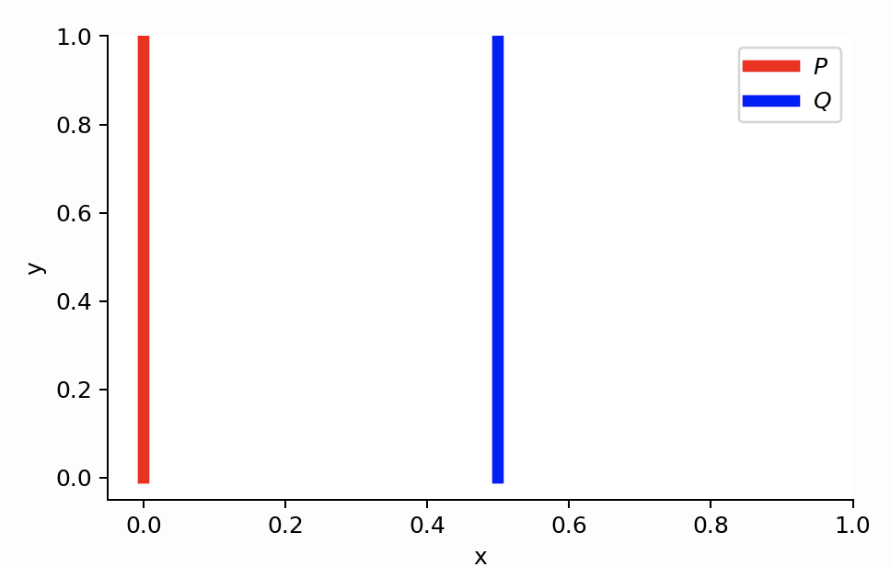
\includegraphics[width=0.8\linewidth]{figs/w_kl_jsd}
		\end{figure}
	\end{minipage}
	\begin{itemize}
		\footnotesize
		\item $\theta = 0$.
		Distributions are the same 
		\[
		KL(\pi || p) = KL(p || \pi) = JSD(p || \pi) = W(\pi, p) = 0
		\]
		\item $\theta \neq 0$
		\[
		KL(\pi || p) = \int_{U[0, 1]} 1 \log \frac{1}{0} d y = \infty = KL(p || \pi)
		\]
		\[
		JSD(\pi || p) = \frac{1}{2}\left( \int_{U[0, 1]}1 \log \frac{1}{1/2} dy + \int_{U[0, 1]}1 \log \frac{1}{1/2} dy \right) = \log 2
		\]
		\[
		W(\pi, p) = |\theta|
		\]
	\end{itemize}
	
	\myfootnote{\href{https://arxiv.org/abs/1904.08994}{Weng L. From GAN to WGAN, 2019} \\ 
		\href{https://arxiv.org/abs/1701.07875}{Arjovsky M., Chintala S., Bottou L. Wasserstein GAN, 2017}}
\end{frame}
%=======
\begin{frame}{Wasserstein distance vs KL vs JSD}
	\begin{block}{Theorem 1}
		Let $\bG_{\btheta}(\bz)$ be (almost) any feedforward neural network, and $p(\bz)$ a prior over $\bz$ such that $\bbE_{p(\bz)} \|\bz\| < \infty$. Then therefore $W(\pi, p)$ is continuous everywhere and differentiable almost everywhere.
	\end{block}
	\begin{block}{Theorem 2}
		Let $\pi$ be a distribution on a compact space $\cX$ and $\{p_t\}_{t=1}^\infty$ be a sequence of distributions on $\cX$. 
		\begin{align}
			KL(\pi || p_t) &\rightarrow 0 \, (\text{or }KL (p_t || \pi) \rightarrow 0) \\
			JSD(\pi || p_t) &\rightarrow 0 \\
			W(\pi || p_t) &\rightarrow 0
		\end{align}
		
		Then, considering limits as $t \rightarrow \infty$, (1) implies (2), (2) implies (3).
	\end{block}
	\myfootnotewithlink{https://arxiv.org/abs/1701.07875}{Arjovsky M., Chintala S., Bottou L. Wasserstein GAN, 2017}
\end{frame}
%=======
\begin{frame}{Wasserstein GAN}
	\begin{block}{Wasserstein distance}
		\vspace{-0.5cm}
		\[
		W(\pi || p) = \inf_{\gamma \in \Gamma(\pi, p)} \bbE_{(\bx, \by) \sim \gamma} \| \bx - \by \| =  \inf_{\gamma \in \Gamma(\pi, p)} \int \| \bx - \by \| \gamma (\bx, \by) d \bx d \by
		\]
		\vspace{-0.3cm}
	\end{block}
	The infimum across all possible joint distributions in $\Gamma(\pi, p)$ is intractable.
	\begin{block}{Theorem (Kantorovich-Rubinstein duality)}
		\vspace{-0.3cm}
		\[
		W(\pi || p) = \frac{1}{K} \max_{\| f \|_L \leq K} \left[ \bbE_{\pi(\bx)} f(\bx)  - \bbE_{p(\bx)} f(\bx)\right],
		\]
		where $f : \bbR^n \rightarrow \bbR$, $\| f \|_L \leq K$ are $K-$Lipschitz continuous functions ($f: \cX \rightarrow \bbR$)
		\vspace{-0.2cm}
		\[
		|f(\bx_1) - f(\bx_2)| \leq K \| \bx_1 - \bx_2 \|, \quad \text{for all } \bx_1, \bx_2 \in \cX.
		\]
		\vspace{-0.6cm}
	\end{block}
	Now we need only samples to get Monte Carlo estimate for $W(\pi || p)$.
	
	\myfootnotewithlink{https://arxiv.org/abs/1701.07875}{Arjovsky M., Chintala S., Bottou L. Wasserstein GAN, 2017}
\end{frame}
%=======
\section{Lipschitzness of Wasserstein GAN critic}
%=======
\subsection{Wasserstein GAN}
%=======
\begin{frame}{Wasserstein GAN}
	\begin{block}{Theorem (Kantorovich-Rubinstein duality)}
		\[
		W(\pi || p) = \frac{1}{K} \max_{\| f \|_L \leq K} \left[ \bbE_{\pi(\bx)} f(\bx)  - \bbE_{p(\bx)} f(\bx)\right],
		\]
	\end{block}
	\begin{itemize}
		\item Now we have to ensure that $f$ is $K$-Lipschitz continuous.
		\item Let $f_{\bphi}(\bx)$ be a feedforward neural network parametrized by~$\bphi$.
		\item If parameters $\bphi$ lie in a compact set $\boldsymbol{\Phi}$ then $f_{\bphi}(\bx)$ will be $K$-Lipschitz continuous function. 
		\item Let the parameters be clamped to a fixed box $\boldsymbol{\Phi} \in [-c, c]^d$ (e.x. $c = 0.01$) after each gradient update.
	\end{itemize}
	\begin{multline*}
		K \cdot W(\pi || p) = \max_{\| f \|_L \leq K} \left[ \bbE_{\pi(\bx)} f(\bx)  - \bbE_{p(\bx)} f(\bx)\right] \geq \\  \geq \max_{\bphi \in \boldsymbol{\Phi}} \left[ \bbE_{\pi(\bx)} f_{\bphi}(\bx)  - \bbE_{p(\bx)} f_{\bphi}(\bx)\right]
	\end{multline*}
	
	\myfootnotewithlink{https://arxiv.org/abs/1701.07875}{Arjovsky M., Chintala S., Bottou L. Wasserstein GAN, 2017}
\end{frame}
%=======
\begin{frame}{Wasserstein GAN}
	\begin{block}{Standard GAN objective}
		\vspace{-0.2cm}
		\[
		\min_{\btheta} \max_{\bphi} \bbE_{\pi(\bx)} \log D_{\bphi}(\bx) + \bbE_{p(\bz)} \log (1 - D_{\bphi}(\bG_{\btheta}(\bz)))
		\]
		\vspace{-0.2cm}
	\end{block}
	\begin{block}{WGAN objective}
		\vspace{-0.3cm}
		\[
		\min_{\btheta} W(\pi || p) \approx \min_{\btheta} \max_{\bphi \in \boldsymbol{\Phi}} \left[ \bbE_{\pi(\bx)} f_{\bphi}(\bx)  - \bbE_{p(\bz)} f_{\bphi}(\bG_{\btheta}(\bz))\right].
		\]
		\vspace{-0.3cm}
	\end{block}
	\begin{itemize}
		\item Discriminator $D$ is similar to the function $f$, but not the same (it is not a classifier anymore). In the WGAN model, function~$f$ is usually called $\textbf{critic}$.
		\item \textit{"Weight clipping is a clearly terrible way to enforce a Lipschitz constraint"}. If the clipping parameter $c$ is too large, it is hard to train the critic till optimality. If the clipping parameter $c$ is too small, it could lead to vanishing gradients.
	\end{itemize}
	
	\myfootnotewithlink{https://arxiv.org/abs/1701.07875}{Arjovsky M., Chintala S., Bottou L. Wasserstein GAN, 2017}
\end{frame}
%=======
\begin{frame}{Wasserstein GAN}
	\begin{minipage}[t]{0.6\columnwidth}
		\begin{itemize}
			\item WGAN has non-zero gradients for disjoint supports.
			\item $JSD(\pi || p)$ correlates poorly with the sample quality. Stays constast nearly maximum value $\log 2 \approx 0.69$.
			\item $W(\pi || p)$ is highly correlated with the sample quality. 
		\end{itemize}
	\end{minipage}%
	\begin{minipage}[t]{0.4\columnwidth}
		\begin{figure}
			\centering
			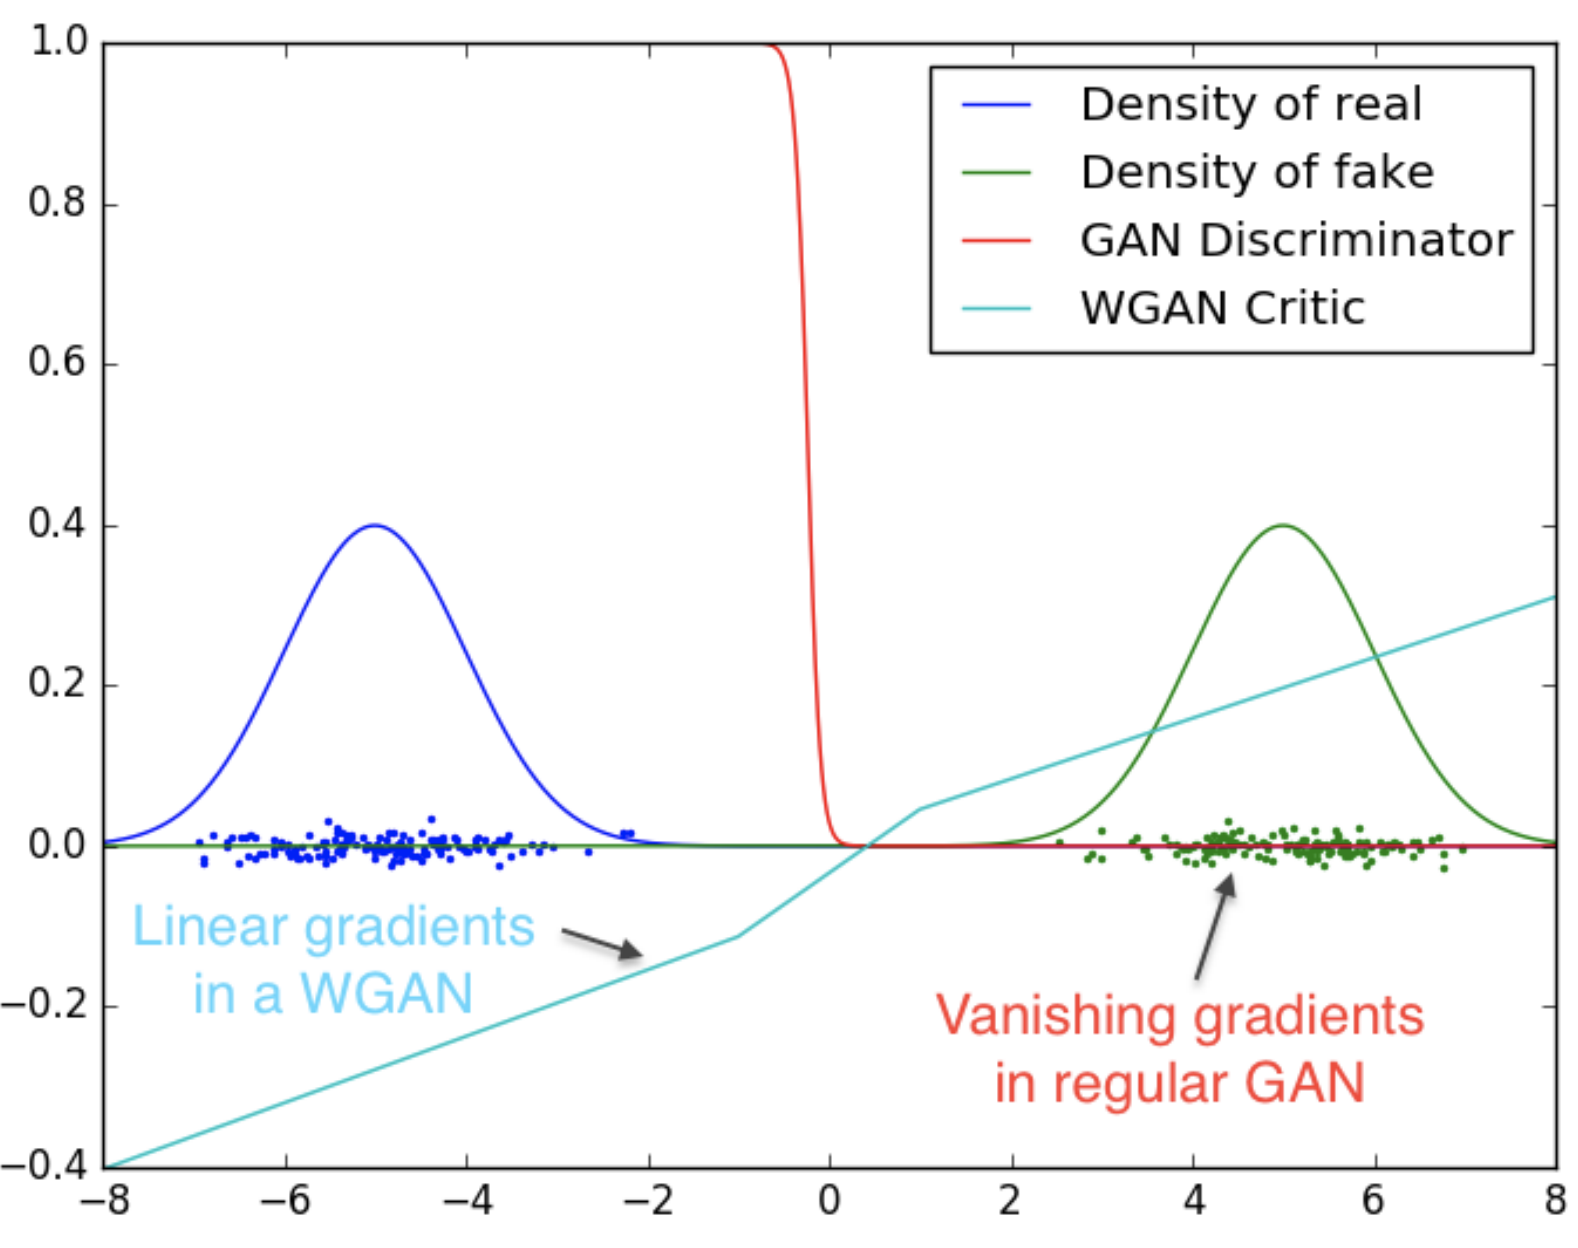
\includegraphics[width=\linewidth]{figs/wgan_toy}
		\end{figure}
	\end{minipage}
	\begin{minipage}[t]{0.5\columnwidth}
		\begin{figure}
			\centering
			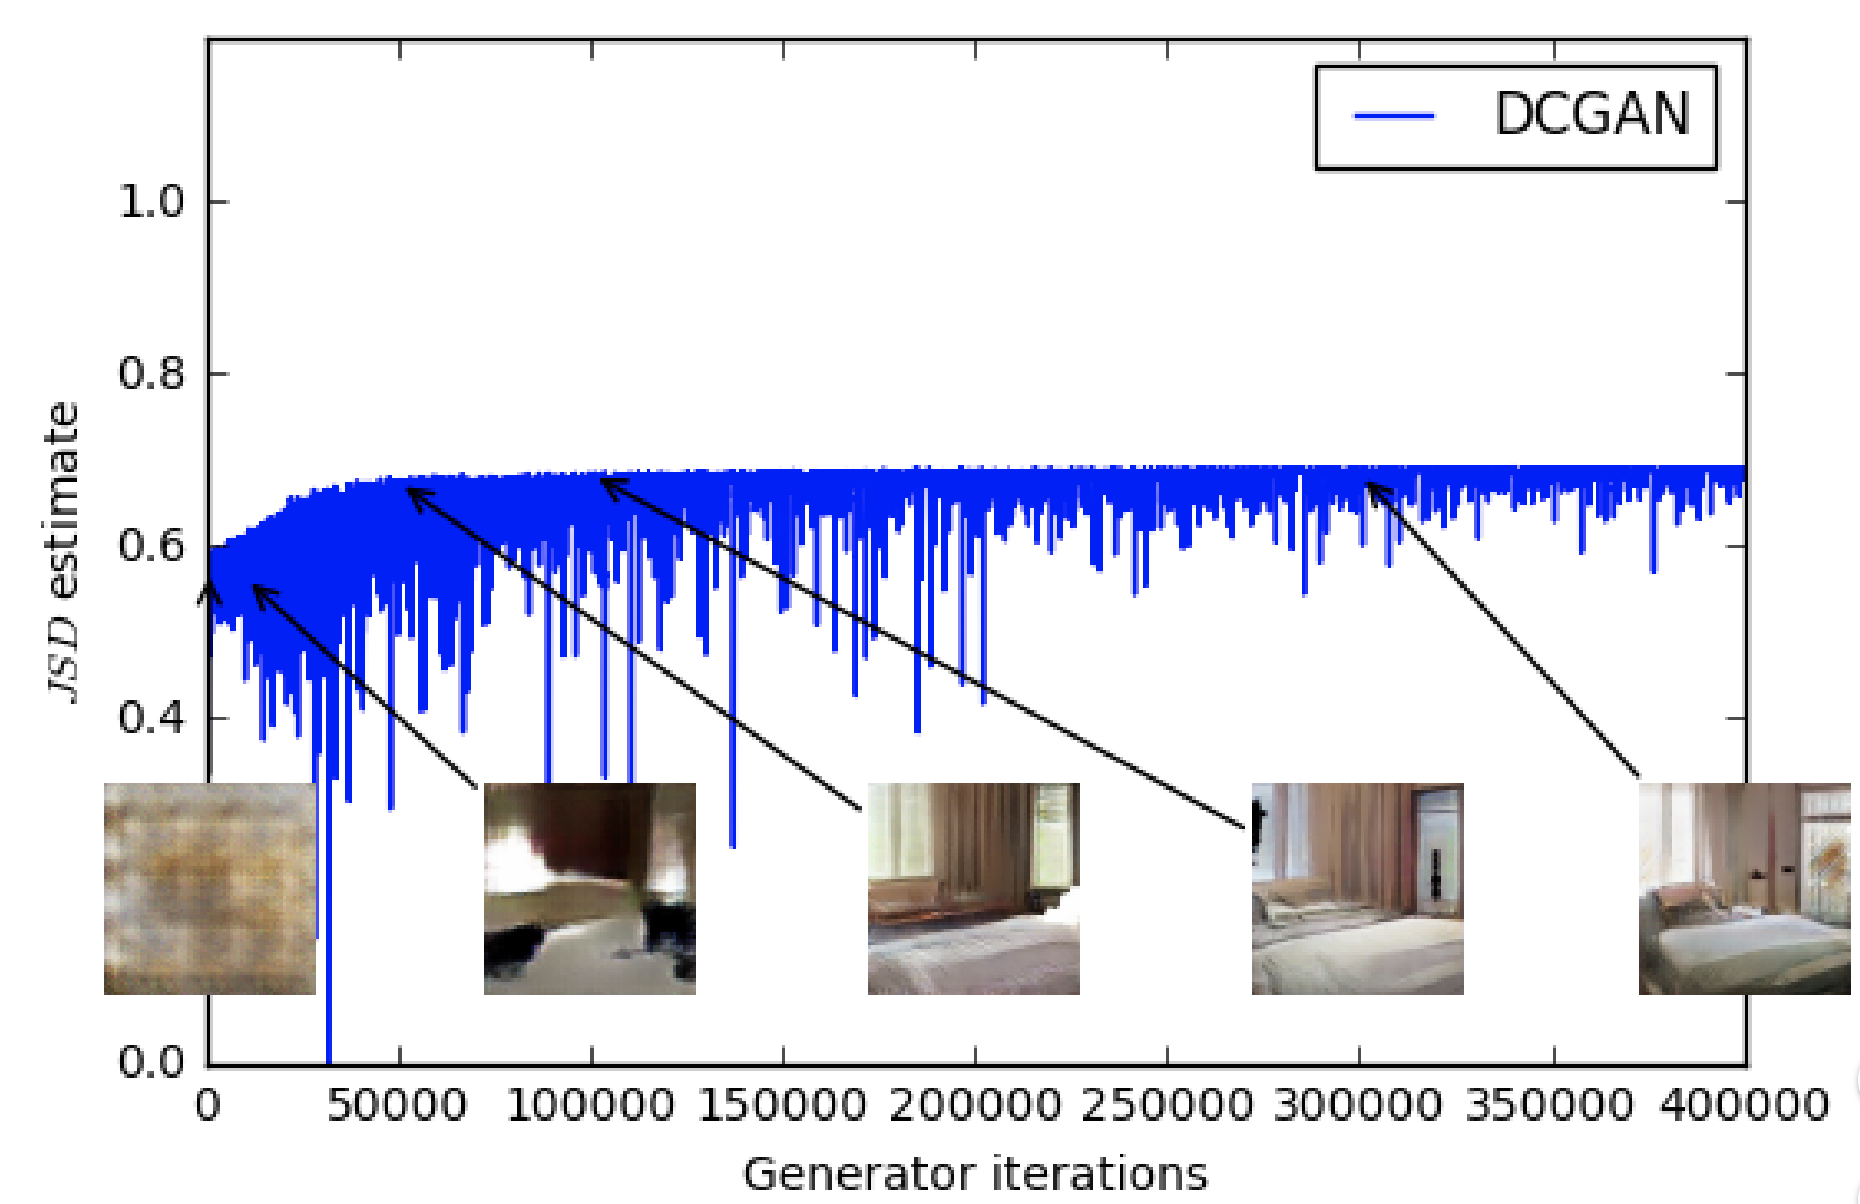
\includegraphics[width=1.0\linewidth]{figs/dcgan_quality}
		\end{figure}
	\end{minipage}%
	\begin{minipage}[t]{0.5\columnwidth}
		\begin{figure}
			\centering
			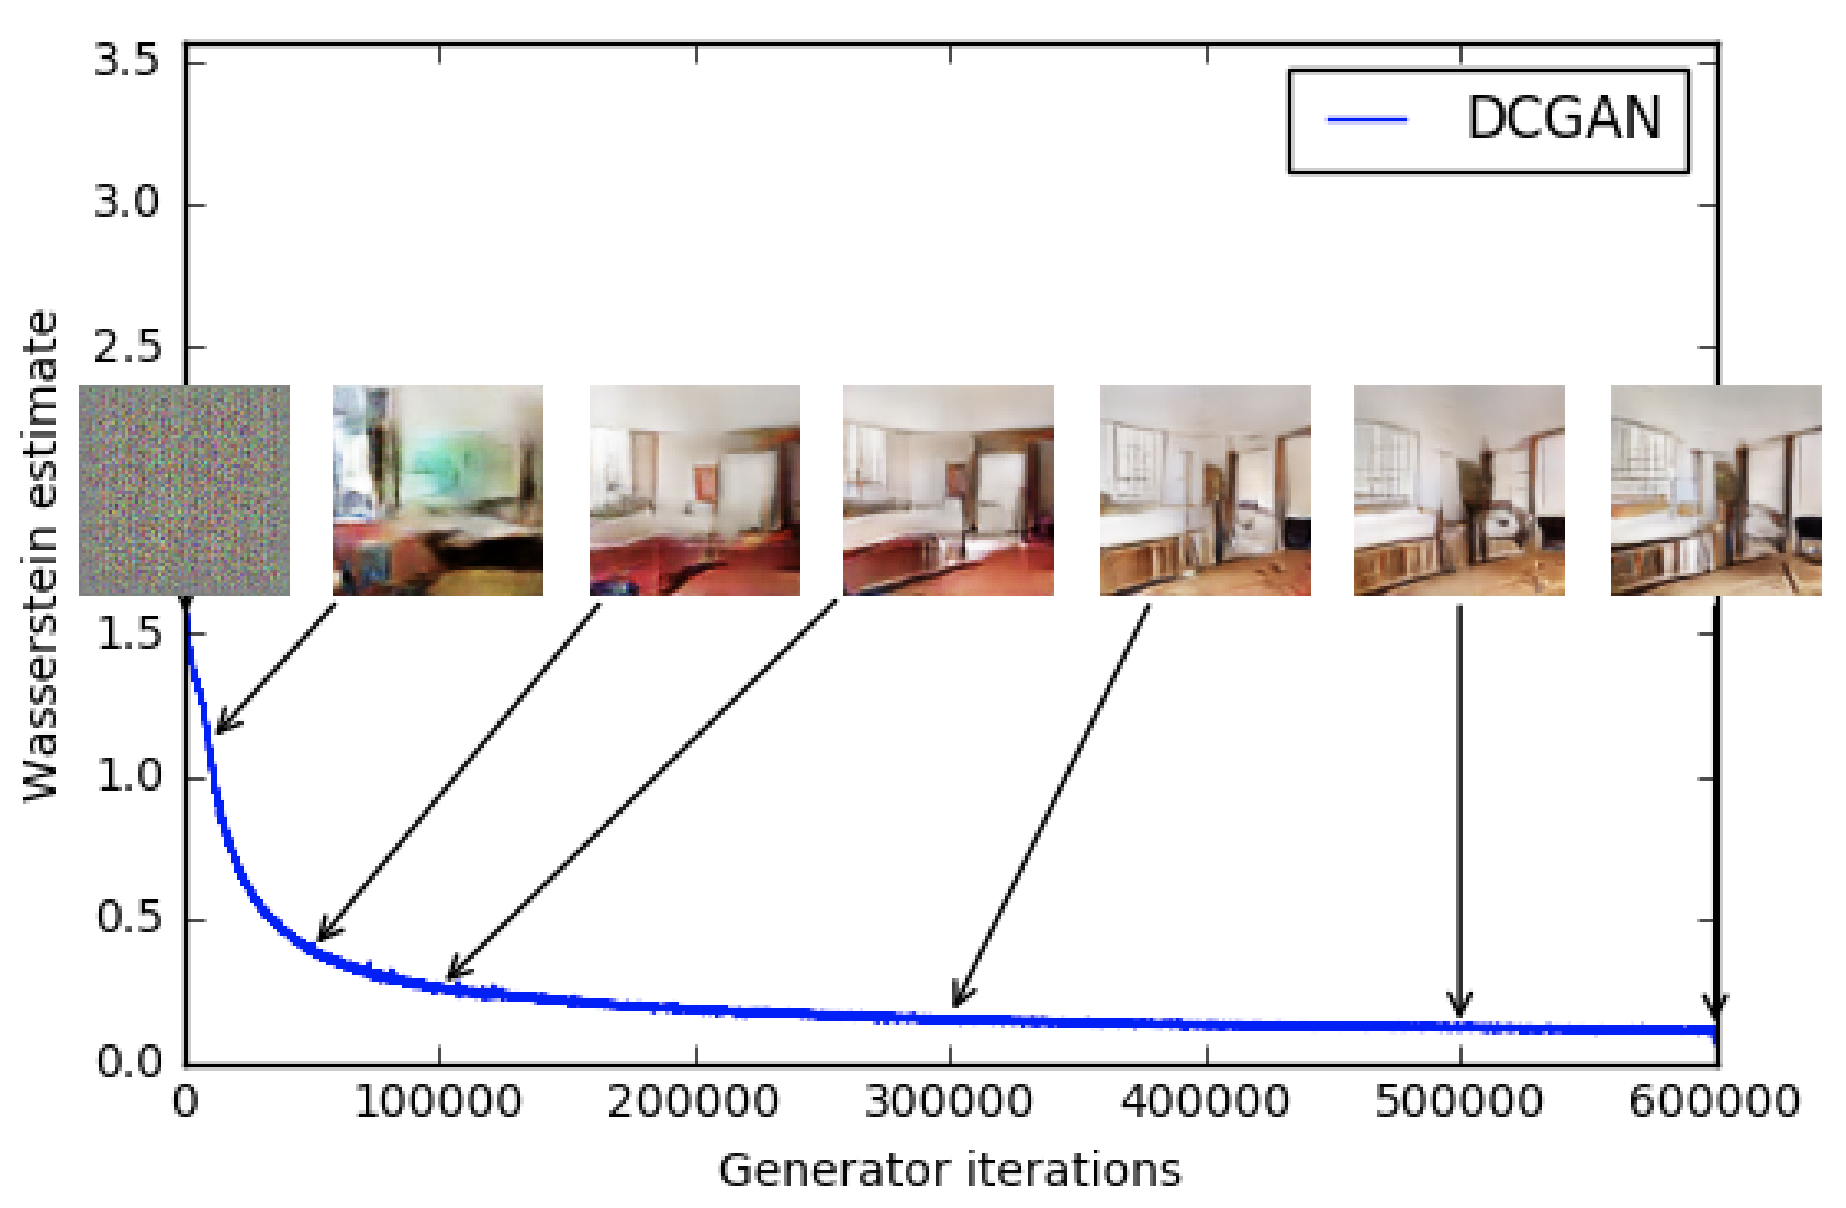
\includegraphics[width=1.0\linewidth]{figs/wgan_quality}
		\end{figure}
	\end{minipage}
	
	\myfootnotewithlink{https://arxiv.org/abs/1701.07875}{Arjovsky M., Chintala S., Bottou L. Wasserstein GAN, 2017}
\end{frame}
%=======
\subsection{WGAN with Gradient Penalty}
%=======
\begin{frame}{Wasserstein GAN with Gradient Penalty}
	\vspace{-0.2cm}
	\begin{figure}
		\centering
		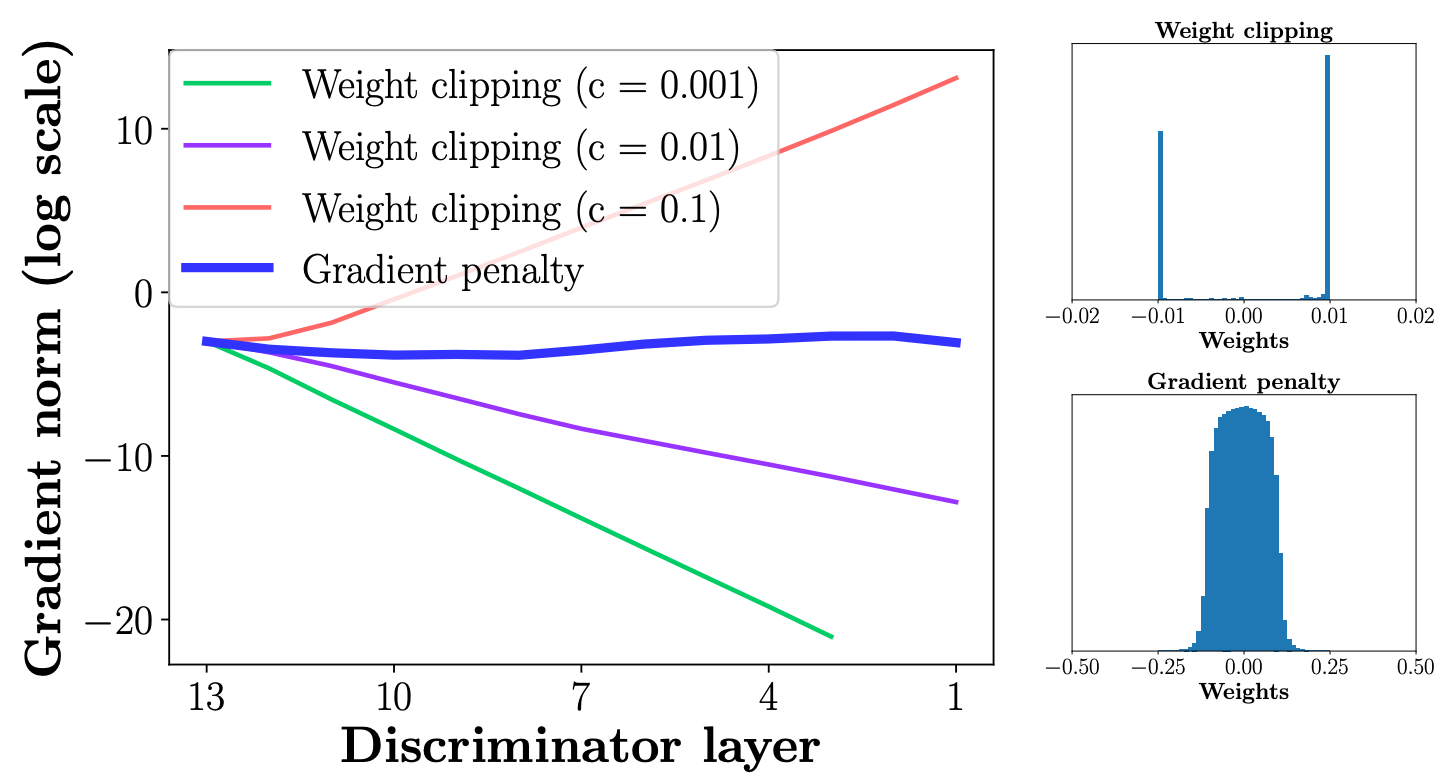
\includegraphics[width=0.9\linewidth]{figs/wgan_gp_weights}
	\end{figure}
	\vspace{-0.2cm} 
	
	\begin{block}{Weight clipping analysis}
		\begin{itemize}
			\item The gradients either grow or decay exponentially.
			\item Gradient penalty makes the gradients more stable.
		\end{itemize}
	\end{block}
	\myfootnotewithlink{https://arxiv.org/abs/1704.00028}{Gulrajani I. et al. Improved Training of Wasserstein GANs, 2017}
\end{frame}
%=======
\begin{frame}{Wasserstein GAN with Gradient Penalty}
	\begin{block}{Theorem}
		Let $\pi(\bx)$ and $p(\bx)$ be two distribution in $\cX$, a compact metric space. Let $\gamma$ be the optimal transportation plan between $\pi(\bx)$ and $p(\bx)$. Then
		\begin{enumerate}
			\item there is 1-Lipschitz function $f^*$ which is the optimal solution of 
			\[
				\max_{\| f \|_L \leq 1} \left[ \bbE_{\pi(\bx)} f(\bx)  - \bbE_{p(\bx)} f(\bx)\right].
			\]
			\item if $f^*$ is differentiable, $\gamma(\by = \bz) = 0$ and $\hat{\bx}_t = t \by + (1 - t) \bz$ with $\by \sim \pi(\bx)$, $\bz \sim p(\bx | \btheta)$, $t \in [0, 1]$ it holds that
			\[
				\bbP_{(\by, \bz) \sim \gamma} \left[ \nabla f^*(\hat{\bx}_t) = \frac{\bz - \hat{\bx}_t}{\| \bz - \hat{\bx}_t \|} \right] = 1.
			\]
		\end{enumerate}
	\end{block}
	\vspace{-0.5cm}
	\begin{block}{Corollary}
		$f^*$ has gradient norm 1 almost everywhere under $\pi(\bx)$ and $p(\bx)$.
	\end{block}

	\myfootnotewithlink{https://arxiv.org/abs/1704.00028}{Gulrajani I. et al. Improved Training of Wasserstein GANs, 2017}
\end{frame}
%=======
\begin{frame}{Wasserstein GAN with Gradient Penalty}
	A differentiable function is 1-Lipschtiz if and only if it has gradients with norm at most 1 everywhere.
	\begin{block}{Gradient penalty}
		\vspace{-0.3cm}
		\[
			W(\pi || p) = \underbrace{\bbE_{\pi(\bx)} f(\bx)  - \bbE_{p(\bx)} f(\bx)}_{\text{original critic loss}} + \lambda \underbrace{\bbE_{U[0, 1]} \left[ \left( \| \nabla f(\hat{\bx}) \|_2 - 1 \right) ^ 2\right]}_{\text{gradient penalty}},
		\]
		\vspace{-0.3cm}
	\end{block}
	\begin{itemize}
		\item Samples $\hat{\bx}_t = t \cdot \by + (1 - t) \cdot \bz$ with $t \in [0, 1]$ are uniformly sampled along straight lines between pairs of points: $\by \sim \pi(\bx)$ and $\bz \sim p(\bx | \btheta)$.
		\item Enforcing the unit gradient norm constraint everywhere is intractable, it turns out to be sifficient to enforce it only along these straight lines.
	\end{itemize}

	\myfootnotewithlink{https://arxiv.org/abs/1704.00028}{Gulrajani I. et al. Improved Training of Wasserstein GANs, 2017}
\end{frame}
%=======
\section{f-divergence minimization}
%=======
\begin{frame}{Divergences}
	\begin{itemize}
		\item Forward KL divergence in maximum likelihood estimation.
		\item Reverse KL in variational inference.
		\item JS divergence in standard GAN.
		\item Wasserstein distance in WGAN.
	\end{itemize}
	\begin{block}{What is a divergence?}
		Let $\cP$ be the set of all possible probability distributions. Then $D: \cP \times \cP \rightarrow \bbR$ is a divergence if 
		\begin{itemize}
			\item $D(\pi || p) \geq 0$ for all $\pi, p \in \cP$;
			\item $D(\pi || p) = 0$ if and only if $\pi \equiv p$.
		\end{itemize}
	\end{block}
	\begin{block}{General divergence minimization task}
		\vspace{-0.3cm}
		\[
			\min_p D(\pi || p)
		\]
		\vspace{-0.7cm}
	\end{block}
	\begin{block}{Chalenge}
		We do not know the real distribution $\pi(\bx)$!
	\end{block}
\end{frame}
%=======
\begin{frame}{f-divergence family}
	
	\begin{block}{f-divergence}
		\vspace{-0.3cm}
		\[
		D_f(\pi || p) = \bbE_{p(\bx)}  f\left( \frac{\pi(\bx)}{p(\bx)} \right)  = \int p(\bx) f\left( \frac{\pi(\bx)}{p(\bx)} \right) d \bx.
		\]
		Here $f: \bbR_+ \rightarrow \bbR$ is a convex, lower semicontinuous function satisfying $f(1) = 0$.
	\end{block}
	\begin{figure}
		\centering
		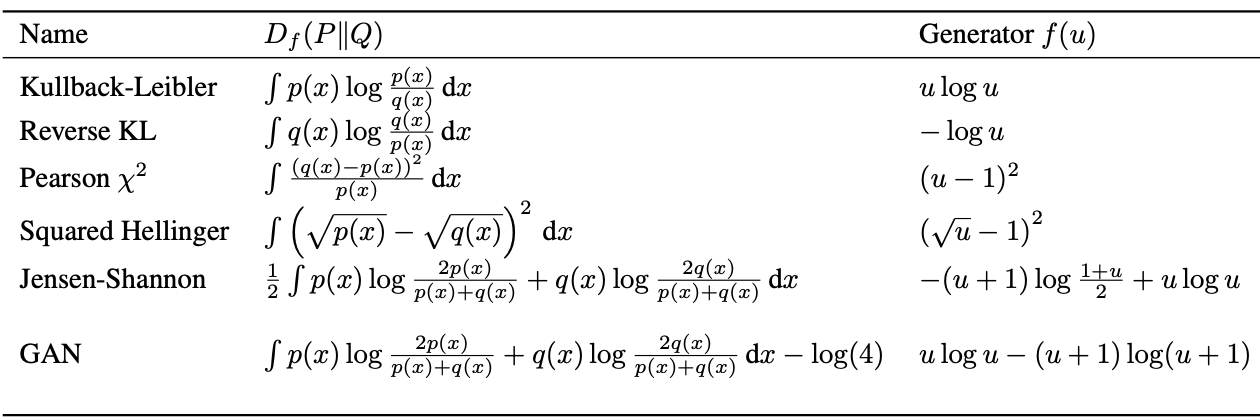
\includegraphics[width=\linewidth]{figs/f_divs}
	\end{figure}
	\myfootnotewithlink{https://arxiv.org/abs/1606.00709}{Nowozin S., Cseke B., Tomioka R. f-GAN: Training Generative Neural Samplers using Variational Divergence Minimization, 2016}
\end{frame}
%=======
\begin{frame}{f-divergence family}
	\vspace{-0.2cm}
	\begin{block}{Fenchel conjugate}
		\vspace{-0.7cm}
		\[
		f^*(t) = \sup_{u \in \text{dom}_f} \left( ut - f(u) \right), \quad f(u) = \sup_{t \in \text{dom}_{f^*}} \left( ut - f^*(t) \right)
		\]
		\vspace{-0.5cm}
	\end{block}
	\textbf{Important property:} $ f^{**} = f$ for convex $f$.
	\begin{block}{f-divergence}
		\vspace{-0.8cm}
		\begin{multline*}
			D_f(\pi || p) = \bbE_{p(\bx)}  f\left( \frac{\pi(\bx)}{p(\bx)} \right)  = \int p(\bx) {\color{violet}f\left( \frac{\pi(\bx)}{p(\bx)} \right) } d \bx = \\ = \int p(\bx) {\color{violet} \sup_{t \in \text{dom}_{f^*}} \left( \frac{\pi(\bx)}{p(\bx)} t - f^*(t) \right)} d \bx = \\ 
			= \int \sup_{t \in \text{dom}_{f^*}} \left( \pi(\bx)t - p(\bx) f^*(t) \right) d \bx .
		\end{multline*}
		\vspace{-0.6cm}
	\end{block}
	Here we seek value of $t$, which gives us maximum value of $ \pi(\bx)t - p(\bx) f^*(t)$, for each data point $\bx$.
	\myfootnotewithlink{https://arxiv.org/abs/1606.00709}{Nowozin S., Cseke B., Tomioka R. f-GAN: Training Generative Neural Samplers using Variational Divergence Minimization, 2016}
\end{frame}
%=======
\begin{frame}{f-divergence family}
	\vspace{-0.4cm}
	\begin{block}{f-divergence}
		\vspace{-0.3cm}
		\[
		D_f(\pi || p) = \bbE_{p(\bx)}  f\left( \frac{\pi(\bx)}{p(\bx)} \right)  = \int p(\bx) f\left( \frac{\pi(\bx)}{p(\bx)} \right) d \bx.
		\]
		\vspace{-0.4cm}
	\end{block}
	\begin{block}{Variational f-divergence estimation}
		\vspace{-0.8cm}
		\begin{multline*}
			D_f(\pi || p)  = {\color{violet}\int} {\color{teal} \sup_{t \in \text{dom}_{f^*}}} \left( \pi(\bx)t - p(\bx) f^*(t) \right) d \bx \geq \\
			 \geq {\color{teal}\sup_{T \in \cT}} {\color{violet}\int} \left( \pi(\bx)T(\bx) - p(\bx) f^*(T(\bx)) \right) d \bx = \\
			 = \sup_{T \in \cT} \left[\bbE_{\pi}T(\bx) -  \bbE_p f^*(T(\bx)) \right]
		\end{multline*}
	\vspace{-0.6cm}
	\end{block}
	This is a lower bound because of Jensen inequality and restricted class of functions $\cT: \cX \rightarrow \bbR$. 
	
	\myfootnotewithlink{https://arxiv.org/abs/1606.00709}{Nowozin S., Cseke B., Tomioka R. f-GAN: Training Generative Neural Samplers using Variational Divergence Minimization, 2016}
\end{frame}
%=======
\begin{frame}{f-divergence family}
	\begin{block}{Variational divergence estimation}
		\[
			D_f(\pi || p) \geq \sup_{T \in \cT} \left[\bbE_{\pi}T(\bx) -  \bbE_p f^*(T(\bx)) \right]
		\]
		The lower bound is tight for $T^*(\bx) = f'\left( \frac{\pi(\bx)}{p(\bx)} \right)$.
	\end{block}
	\begin{block}{Example (JSD)}
		\begin{itemize}
			\item Let define function $f$ and its conjugate $f^*$
			\[ 
				f(u) = u \log u - (u + 1) \log (u + 1), \quad f^*(t) = - \log (1 - e^t).
			\]
			\item Let reparametrize $T(\bx) = \log D(\bx)$.
		\end{itemize}
		\vspace{-0.4cm}
	\end{block}
	\[
		\min_{G} \max_D \left[ \bbE_{\pi(\bx)} \log D(\bx) + \bbE_{p(\bz)} \log (1 - D(\bG(\bz))) \right]
	\]

	\myfootnotewithlink{https://arxiv.org/abs/1606.00709}{Nowozin S., Cseke B., Tomioka R. f-GAN: Training Generative Neural Samplers using Variational Divergence Minimization, 2016}
\end{frame}
%=======
\begin{frame}{f-divergence family}
	\begin{block}{Variational divergence estimation}
		\[
			D_f(\pi || p) \geq \sup_{T \in \cT} \left[\bbE_{\pi}T(\bx) -  \bbE_p f^*(T(\bx)) \right]
		\]
	\end{block}
	\textbf{Note:} To evaluate lower bound we only need samples from $\pi(\bx)$ and $p(\bx)$. Hence, we could fit implicit generative model.
	\begin{figure}
		\centering
		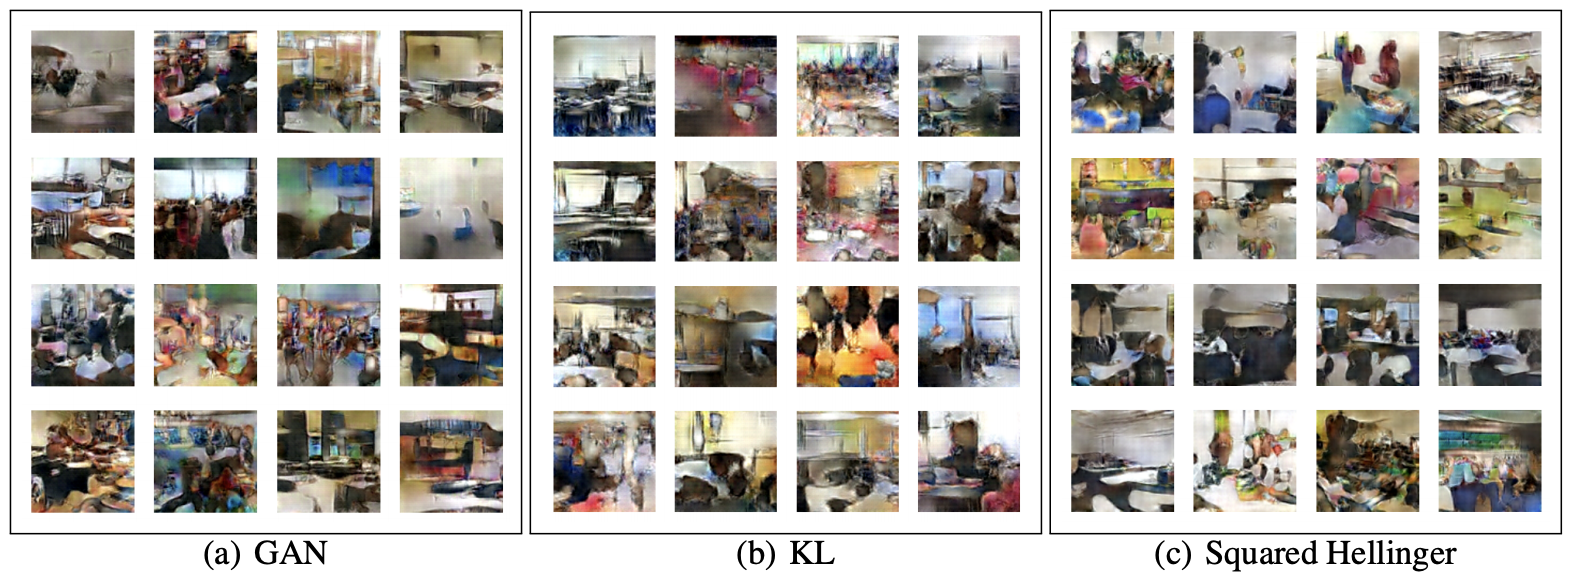
\includegraphics[width=1.0\linewidth]{figs/f_div_results}
	\end{figure}

	\myfootnotewithlink{https://arxiv.org/abs/1606.00709}{Nowozin S., Cseke B., Tomioka R. f-GAN: Training Generative Neural Samplers using Variational Divergence Minimization, 2016}
\end{frame}
%=======
\begin{frame}{Summary}
	\begin{itemize}
		\item KL and JS divergences work poorly as model objective in the case of disjoint supports.
		\vfill
		\item Earth-Mover distance is a more appropriate objective function for distribution matching problem.	
		\vfill
		\item Kantorovich-Rubinstein duality gives the way to calculate the EM distance using only samples.
		\vfill
		\item Wasserstein GAN uses Kantorovich-Rubinstein duality for getting Earth Mover distance as model objective.
		\vfill
		\item Weight clipping is a terrible way to enforce Lipschitzness. Gradient Penalty adds regularizer to loss that uses neccessary conditions for optimal critic. 	
		\vfill
		\item f-divergence family is a unified framework for divergence minimization, which uses variational approximation. Standard GAN is a special case of it.
	\end{itemize}
\end{frame}
%=======
\end{document} 